\documentclass[11pt,a4paper]{article}

\usepackage[utf8]{inputenc}
\usepackage[T1]{fontenc}
\usepackage[english]{babel}
\usepackage{verbatim}
\usepackage{amsfonts}
\usepackage{amssymb}

\usepackage{amsmath}
\DeclareMathOperator*{\argmax}{argmax}
\DeclareMathOperator*{\argmin}{argmin}
\DeclareMathOperator*{\med}{med}

\usepackage{amsthm}
\usepackage{graphicx}
\usepackage{lmodern}
\usepackage{empheq}
\usepackage{epsfig}
\usepackage{tikz}
\usepackage{xcolor}
\usepackage{algorithm}
\usepackage{algorithmic}
\usepackage{fancyvrb}
\usepackage{moreverb}
\usepackage{listings}
\usepackage{url}
%%\usepackage[round]{natbib}

\setlength{\unitlength}{1mm}
\usepackage{pstricks}

\usepackage[top=3cm, bottom=3cm, left=3cm, right=3cm]{geometry}

%%\usepackage{hyperref}

\begin{document}
\section{Introduction}
While many algorithm for learning from demonstration are based on training data, we propose to leverage the interaction between the teacher and learner. We believe that learning from demonstration with natural interaction has many advantages. It allows easy reprogramming of the robot since data acquisition in laboratory framework is not necessary. Moreover, the robot can interrupt the demonstration and engage in an interaction with the teacher in order to disambiguate its understanding, reducing the amount of data needed for learning.
\newline
In order to allow natural interaction, we rely on non-intrusive recording systems. Teaching from demonstration involves many communication cues. The language informed about the objects and the task to perform nevertheless other non-verbal communication cues carry those informations too. In particular, the gaze is an important one. 
\newline
The gaze informs about attention and intention. Therefore, it can be used as a prior for task segmentation and recognition. The estimation of the gaze relies on the algorithm presented in \cite{Funes2016} where the gaze is infrared from RGB and Depth video steams obtained from a Microsoft Kinect.

\section{Motivation}
The present dataset would be used to evaluate the gaze estimation algorithm. As a first step, we aim to evaluate the accuracy of the gaze estimation algorithm using a controlled (supervised) calibration procedure. In a second step, we use the human-robot interactions to infer unsupervised calibration method. In particular, we are interested in calibration methods using interaction cues to infer the calibration targets. Moreover, we are interesting in the inference of calibration target based on object geometry. Finally, we aim to leverage gaze behavior during demonstration. In particular, the segmentation and recognition of the demonstration. For more details on the proposed benchmarks refer to section~\ref{Benchmarks}.
\subsection{Gaze calibration}
The gaze calibration procedure relies on the inference of a target for calibration. In the case of point (marker) targets, the target is trivially defined. The present data set aim to provide enough calibration points to evaluate the gaze estimation algorithm with calibration. Nevertheless, the inference of the gaze target is less trivial when the object of attention is big with respect to some dimensions. We will be interesting to evaluate the effect of the gaze calibration procedure while the target is an object (of various size and shape).
\subsection{Gaze behavior}
Based on the accuracy of the gaze estimation algorithm, we would like to leverage some gaze behaviors. In particular, we evaluate how well the gaze estimation algorithm can inferred the Visual Focus Of Attention (VFOA). Further, we would like to incorporate the VFOA model in a multi-modal task segmentation and recognition methods. In particular, we are interesting in the timing of the VFOA to infer demonstration segmentation and recognition.

\section{Data collection}
\label{Data_Collection}
In this section we first describe our recording methotology and then describe the different recording sessions constituting the dataset.
\subsection{Overview}
\label{Overview}
\begin{figure}[!ht]
\begin{center}
\includegraphics[scale=0.05, angle=-90]{Pictures/Baxter_Setup.jpg}
\end{center}
\caption{Experimental setup. \label{Experimental_Setup}}
\end{figure}
The recording setup is as shown in figure \ref{Experimental_Setup}. It comprises and RGB-D camera (a Microsoft Kinect v2), a robot (a Baxter from Rethink Robotics), a table with marker, a cup, a saucer,.... The characteristics and purpose or function of each element are described as follows:
\begin{itemize}
\item Microsoft Kinect v2: this consumer device provides standard video (RGB) and Depth video steams. The RGB camera has an HD resolution ($1920 \times 1080$) while the Depth camera has a resolution of $512 \times 424$. The acquisition rate is 30 frame-per-second.
\item Baxter robot: this is a human like robot from Rethink Robotics. We will use the robot's ego-motion to infer gaze target. In particular, the position of the head of the robot (screen) and its end-effectors are recored.
\item Table with markers: those markers are used as calibration targets for the gaze. Moreover, the object are placed on those markers in order to infer there position without the need of an object detection algorithm. The markers are numbered in order to differentiate them.
\item Cup and Saucer: those object are involved in the demonstration task. We provide a 3D mesh of this objects.
\item Other Objects: those objects are used as gaze target for calibration. We provide a 3D mesh for each objects.
\end{itemize}

\section{Recording sessions}
In order to evaluate the gaze estimation algorithm and calibration, we designed a set of three recording sessions using respectively the end-effector of the robot, the markers on the table and the objects on the table as calibration points. In order to evaluate the gaze estimation algorithm to infer gaze behavior, we designed a set of three recording sessions. In the present section we describe the six recording session.
\subsection{Gaze calibration}
In the present section are described the recording session for the supervised gaze calibration method. It involves three different type target (end-effectors, markers, objects) and two kind of head pose activity (static, natural).
\subsubsection{Targets}
\begin{itemize}
\item \textit{End-Effector (ET)}: the end-effector of the robot is used as a target for calibration. The exact point at which the participants have to look is leverage by a white rubber band on the gripper. For each robot's limbs, the calibration points are contains in a parallelepiped of width and height of 1 meter and depth of 30 centimeters at the left and right of the robot. There are 12 points for both sides of the robot distributed as a grid ($2 \times 3 \times 3$).
\item \textit{Markers Target (MT)}: (need some measurement and camera orientation.) the table is marked with 15 markers distributed as a grid ($3 \times 5$). Each markers is numbered. The experimental supervisor will ask to the participant to look at a marker number until s/he ask her/him to look at the next target.
\item \textit{Object Target (OT)}: the objects are placed on the table (on the markers). The participant start by looking at the robot who asked to the participant to look at on of the object on the table until it asked to stopped and look back to the robot. The robot ask to look at an other object and so on. For this experiment, we consider only the natural head pose activity framework.
\end{itemize}
\subsubsection{Head pose activity}
\begin{itemize}
\item \textit{Static Pose (SP)}: the participant start by looking at the middle of the robot's screen in order to guarantee frontal view of the face. Then, the participant is asked to keep his head pose fixed.
\item \textit{Natural Pose (NP)}: The participant can freely move its head toward the target.
\end{itemize}
\subsection{Gaze behavior}
\begin{itemize}
\item \textit{Robot Interaction (RI)}: Baxter says "Hi." and stretches its hand for a shake and says "How are you?". It waits for the shake and brings its hands back.
\item \textit{Cup and saucer Interaction (CI)}: the cup and the saucer are placed on two table markers. The participant has to take the cup and place it on the saucer. Then, s/he takes the saucer (with the cup on) and place on a the defined marker. Each participants proceed to 3 different setup.
\item \textit{Table Interaction (TI)}: Put the table (dishes, fork, knife, glass).
\end{itemize}

\subsection{Remarks}
In order to not bias the natural gaze behavior of the participants, we proceed first with the gaze behavior experiment and, then, with the gaze calibration.

\section{Data processing}
Besides the raw data describe in section \ref{Overview}, we also provide additional information that is essential for deriving ground truth measures for evaluation or simply useful to exploit the dataset and run the experiments. It compromises the camera calibration, the synchronization, the head pose, the manual annotations, the target position, and 3D object meshes. Below, we present the procedure to estimate those parameters

\subsection{World coordinate system definition}
To standardize the definition all 3D variable in the data, we have defined a common world coordinate system (WCS), in which the variable refers to \textit{meters}. It has been define as the robot frame being at the base of the robot.

\subsection{RGB-D sensors intrinsic calibration}
For the calibration of the Microsoft Kinect v2, we rely on the \texttt{iai\_kinect} softwares. It computes the intrinsic of the RGB and Depth camera, as well as the extrinsic parameters between both cameras.

\subsection{RGB-D sensors extrinsic calibration and synchrony}
The rigid transform from the robot to the camera frame can be evaluated using the position of the end-effector in the RGB-D camera. The synchronization of the robot and camera use done by time-stamping the robot time with the computer and using the \texttt{MessageFilter} ROS package.

\subsection{Target position}
By placing the object on the markers of the table, one can evaluate there position when there are on the table. In the future, we will provide object position using our 3D meshes of the object or an other methods based on object detection. Nevertheless, we have to provide a ground truth for the gaze during OT (in particular). We ask to the participants which part of the object they look at. We report those region on pictures of the object. The position of the target is given for each frame. Each object has its own ID which is given in the data set. Moreover, an additional variable is set to "left", "right" or "NA" if the object is manipulated, respectively, by the left, the right hand or is not manipulated.

\subsection{Body landmark}
We will report body landmark position as hands, shoulders and head pose using our tracker (REFERENCE).

\subsection{Gaze behavior label}
Each frame is labeled with a "b" when the participant is blinking. The frame is labeled by the object ID when the participant is looking at the object. In the case of saccade or undefined VFOA (gaze search), the frame is labeled with "NA". This labeling is done manually. 
\paragraph{Remark}
For the RT recording, the target is not visible in the RGB stream. Therefore, it is difficult to label the gaze at the end-effector. One could to the labelling during the recording when the supervisor has a complete view of the scene. Another possibility consists in recording again if the participant has been distracted. The check is done during the recording.

\section{Benchmarks}
\label{Benchmarks}
In present section, we describe different evaluation benchmarks for gaze calibration, as well as for gaze behavior and task segmentation and recognition.
\subsection{Benchmark 1: Natural versus Static head pose activity}
\subsection{Benchmark 2: RT versus MT} 
\subsection{Benchmark 3: MT versus OT}
\subsection{Benchmark 4: RT versus OT}
\subsection{Benchmark 5: RI versus RT, MT and OT}
\subsection{Benchmark 6: Task segmentation and recognition (CI, TI)}
In our experiments, the tasks consist of pick and place actions. We will characterize a pick and place action by: the object ID, the final position (Gaussian) of the object, a boolean that state if the orientation of the object matters when carrying it, and the timestamps of each step.
\paragraph{Remark} The object position while manipulated is given by the hand position.

\section{Unsupervised gaze calibration}
\begin{figure}[!ht]
\begin{center}
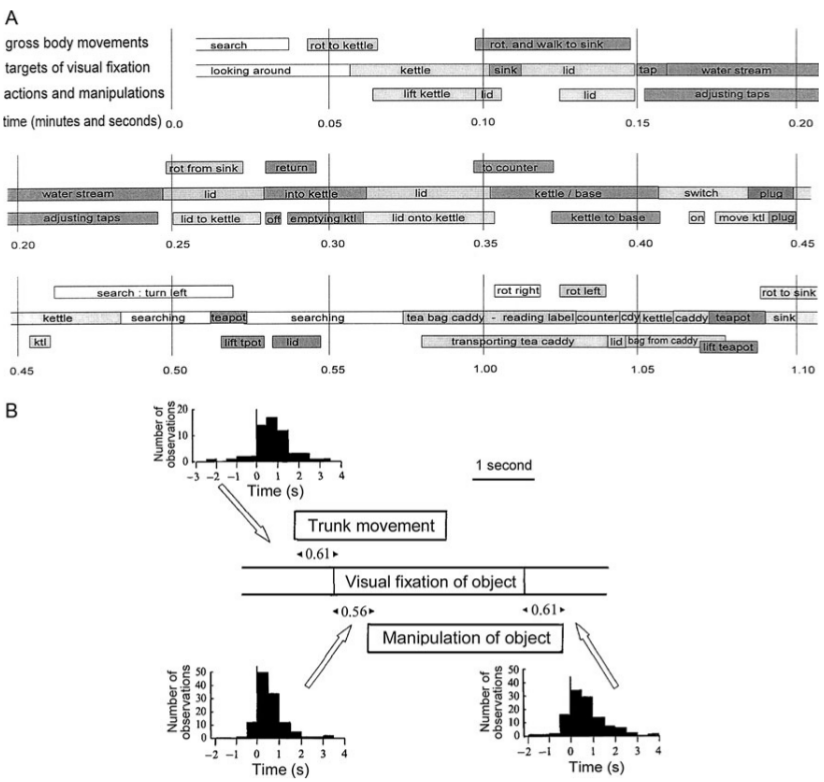
\includegraphics[scale=0.5]{Pictures/GazeObjectBehavior_Land.png}
\end{center}
\caption{Results from \cite{Land2009}. (\textbf{A}) The relative timings of body movements, fixations on particular objects, and manipulation of those objects by the hands during the first 70 s of a tea-making session.
(\textbf{B}) Average relative timings of trunk movements,
fixations on particular objects (which may involve several individual fixations), and manipulation of those objects. The data represent
94 object-related actions from three subjects. Typical actions last about 3 s (extended waiting periods, such as watching for the kettle to
boil, have been excluded). Note that trunk movements (when present) precede fixations, which precede manipulation, by about 0.6 s in
each case. Similarly, fixation moves on to the next object about 0.6 s before manipulation is complete. There are wide variations in timing
(histograms), with manipulation sometimes preceding gaze fixation.\label{LandResults}}
\end{figure}

\clearpage
\bibliographystyle{ieeetr}
\bibliography{Notes}

\end{document}